\documentclass[aspectratio=169]{beamer}
\usetheme{simple}

\RequirePackage[l2tabu, orthodox]{nag}


% \usepackage[left=1.in, right=1.in, top=1.25in, bottom=1.25in]{geometry}

% FONTS
%\usepackage[T1]{fontenc}

% Replace default Latin Modern typewriter with its proportional counterpart
% http://www.tug.dk/FontCatalogue/lmoderntypewriterprop/
%\renewcommand*\ttdefault{lmvtt}


%%% OPTION 1 - Fourier Math + New Century Schoolbook + ParaType Sans

% % Import Fourier Math (this imposes its own New Century Schoolbook type)
% % http://www.ctan.org/tex-archive/fonts/fouriernc/
%\usepackage{fouriernc}
%\usepackage{amsmath}
% % Replace with TeX Gyre Schola version of New Century Schoolbook (must scale!)
% % http://www.tug.dk/FontCatalogue/tgschola/
%\usepackage[scale=0.92]{tgschola}
%\usepackage[scaled=0.88]{PTSans}

%% OPTION 2 - MathDesign Math + Bitstream Charter + ParaType Sans

% Import MathDesign (this brings along Bitstream Charter)
% http://www.ctan.org/tex-archive/fonts/mathdesign/
\usepackage[bitstream-charter]{mathdesign}
\usepackage{amsmath}
\usepackage[scaled=0.92]{PTSans}


% %%% OPTION 3 - MTPRO 2 Math + Termes Times + ParaType Sans

% \usepackage{tgtermes}
% \usepackage{amsmath}
% \usepackage[subscriptcorrection,
%             amssymbols,
%             mtpbb,
%             mtpcal,
%             nofontinfo  % suppresses all warnings
%            ]{mtpro2}
% \usepackage{scalefnt,letltxmacro}
% \LetLtxMacro{\oldtextsc}{\textsc}
% \renewcommand{\textsc}[1]{\oldtextsc{\scalefont{1.10}#1}}
% \usepackage[scaled=0.92]{PTSans}

% Use default fonts here
\usepackage{amsmath}
\usepackage{amssymb}

% \usepackage{titling}

% % COLOR
% \usepackage[table,usenames,dvipsnames]{xcolor}
\definecolor{shadecolor}{gray}{0.9}

% SPACING and TEXT
\usepackage[final,expansion=alltext]{microtype}
\usepackage[english]{babel}
\usepackage[parfill]{parskip}
\usepackage{afterpage}
\usepackage{framed}
\usepackage{verbatim}
\usepackage{setspace}

\newenvironment{exercise}[1]
{
    \itshape
    \paragraph{Exercise: \textit{#1}}
}
{ 
}


% \usepackage[bottom]{footmisc}
\usepackage[symbol]{footmisc}
\renewcommand{\thefootnote}{\arabic{footnote}}


% FIGURES
\usepackage{graphicx}
\usepackage[labelfont={it, small}, 
            textfont={small,singlespacing},
            % justification={justified,RaggedRight},
            singlelinecheck=false,
            margin=0pt]{caption}
\usepackage[format=hang]{subcaption}
% \usepackage{ccaption}

% % APPENDIX FIGURES
% \usepackage{chngcntr}

% % TABLES
% \usepackage{booktabs}
% \usepackage{longtable}
% \usepackage{hhline}

% ALGORITHMS
\usepackage[algoruled]{algorithm2e}
\usepackage{listings}
\usepackage{fancyvrb}
\fvset{fontsize=\normalsize}

% % THEOREMS
\usepackage{amsthm}
\newtheorem{proposition}{Proposition}
% \newtheorem{lemma}{Lemma}

% % BIBLIOGRAPHY
\usepackage{natbib}

% HYPERREF
% \usepackage[colorlinks,linktoc=all]{hyperref}
% \usepackage[all]{hypcap}
% \hypersetup{citecolor=MidnightBlue}
% \hypersetup{linkcolor=black}
% \hypersetup{urlcolor=MidnightBlue}

% % CLEVEREF must come after HYPERREF
% \usepackage[nameinlink]{cleveref}

% % ACRONYMS
% \usepackage[acronym,smallcaps,nowarn]{glossaries}
% % \makeglossaries

% % COLOR DEFINITIONS
\newcommand{\red}[1]{\textcolor{BrickRed}{#1}}
\newcommand{\orange}[1]{\textcolor{BurntOrange}{#1}}
\newcommand{\green}[1]{\textcolor{OliveGreen}{#1}}
\newcommand{\blue}[1]{\textcolor{MidnightBlue}{#1}}
\newcommand{\gray}[1]{\textcolor{black!60}{#1}}

% LISTINGS DEFINTIONS
\lstdefinestyle{mystyle}{
    commentstyle=\color{OliveGreen},
    keywordstyle=\color{BurntOrange},
    numberstyle=\tiny\color{black!60},
    stringstyle=\color{MidnightBlue},
    basicstyle=\ttfamily,
    breakatwhitespace=false,
    breaklines=true,
    captionpos=b,
    keepspaces=true,
    numbers=left,
    numbersep=5pt,
    showspaces=false,
    showstringspaces=false,
    showtabs=false,
    tabsize=2
}
\lstset{style=mystyle}

\usepackage[colorinlistoftodos,
            prependcaption,
            textsize=small,
            backgroundcolor=yellow,
            linecolor=lightgray,
            bordercolor=lightgray]{todonotes}

\usepackage{soul}

\usepackage{media9}
% !TEX root = template.tex

% \DeclareRobustCommand{\mb}[1]{\ensuremath{\boldsymbol{\mathbf{#1}}}}
\DeclareRobustCommand{\mb}[1]{\boldsymbol{#1}}

% \newcommand{\KL}[2]{\ensuremath{\textrm{KL}\PARENS{#1\;\|\;#2}}}
\DeclareRobustCommand{\KL}[2]{\ensuremath{D_{\textrm{KL}}\left(#1\;\|\;#2\right)}}

\DeclareMathOperator*{\argmax}{arg\,max}
\DeclareMathOperator*{\argmin}{arg\,min}

\renewcommand{\mid}{~\vert~}
\newcommand{\given}{\,|\,}
\newcommand{\iid}[1]{\stackrel{\text{iid}}{#1}}

\newcommand{\mba}{\mb{a}}
\newcommand{\mbb}{\mb{b}}
\newcommand{\mbc}{\mb{c}}
\newcommand{\mbd}{\mb{d}}
\newcommand{\mbe}{\mb{e}}
% \newcommand{\mbbf}{\mb{f}}
\newcommand{\mbg}{\mb{g}}
\newcommand{\mbh}{\mb{h}}
\newcommand{\mbi}{\mb{i}}
\newcommand{\mbj}{\mb{j}}
\newcommand{\mbk}{\mb{k}}
\newcommand{\mbl}{\mb{l}}
\newcommand{\mbm}{\mb{m}}
\newcommand{\mbn}{\mb{n}}
\newcommand{\mbo}{\mb{o}}
\newcommand{\mbp}{\mb{p}}
\newcommand{\mbq}{\mb{q}}
\newcommand{\mbr}{\mb{r}}
\newcommand{\mbs}{\mb{s}}
\newcommand{\mbt}{\mb{t}}
\newcommand{\mbu}{\mb{u}}
\newcommand{\mbv}{\mb{v}}
\newcommand{\mbw}{\mb{w}}
\newcommand{\mbx}{\mb{x}}
\newcommand{\mby}{\mb{y}}
\newcommand{\mbz}{\mb{z}}

\newcommand{\mbA}{\mb{A}}
\newcommand{\mbB}{\mb{B}}
\newcommand{\mbC}{\mb{C}}
\newcommand{\mbD}{\mb{D}}
\newcommand{\mbE}{\mb{E}}
\newcommand{\mbF}{\mb{F}}
\newcommand{\mbG}{\mb{G}}
\newcommand{\mbH}{\mb{H}}
\newcommand{\mbI}{\mb{I}}
\newcommand{\mbJ}{\mb{J}}
\newcommand{\mbK}{\mb{K}}
\newcommand{\mbL}{\mb{L}}
\newcommand{\mbM}{\mb{M}}
\newcommand{\mbN}{\mb{N}}
\newcommand{\mbO}{\mb{O}}
\newcommand{\mbP}{\mb{P}}
\newcommand{\mbQ}{\mb{Q}}
\newcommand{\mbR}{\mb{R}}
\newcommand{\mbS}{\mb{S}}
\newcommand{\mbT}{\mb{T}}
\newcommand{\mbU}{\mb{U}}
\newcommand{\mbV}{\mb{V}}
\newcommand{\mbW}{\mb{W}}
\newcommand{\mbX}{\mb{X}}
\newcommand{\mbY}{\mb{Y}}
\newcommand{\mbZ}{\mb{Z}}

\newcommand{\mbalpha}{\mb{\alpha}}
\newcommand{\mbbeta}{\mb{\beta}}
\newcommand{\mbdelta}{\mb{\delta}}
\newcommand{\mbepsilon}{\mb{\epsilon}}
\newcommand{\mbchi}{\mb{\chi}}
\newcommand{\mbeta}{\mb{\eta}}
\newcommand{\mbgamma}{\mb{\gamma}}
\newcommand{\mbiota}{\mb{\iota}}
\newcommand{\mbkappa}{\mb{\kappa}}
\newcommand{\mblambda}{\mb{\lambda}}
\newcommand{\mbmu}{\mb{\mu}}
\newcommand{\mbnu}{\mb{\nu}}
\newcommand{\mbomega}{\mb{\omega}}
\newcommand{\mbphi}{\mb{\phi}}
\newcommand{\mbpi}{\mb{\pi}}
\newcommand{\mbpsi}{\mb{\psi}}
\newcommand{\mbrho}{\mb{\rho}}
\newcommand{\mbsigma}{\mb{\sigma}}
\newcommand{\mbtau}{\mb{\tau}}
\newcommand{\mbtheta}{\mb{\theta}}
\newcommand{\mbupsilon}{\mb{\upsilon}}
\newcommand{\mbvarepsilon}{\mb{\varepsilon}}
\newcommand{\mbvarphi}{\mb{\varphi}}
\newcommand{\mbvartheta}{\mb{\vartheta}}
\newcommand{\mbvarrho}{\mb{\varrho}}
\newcommand{\mbxi}{\mb{\xi}}
\newcommand{\mbzeta}{\mb{\zeta}}

\newcommand{\mbDelta}{\mb{\Delta}}
\newcommand{\mbGamma}{\mb{\Gamma}}
\newcommand{\mbLambda}{\mb{\Lambda}}
\newcommand{\mbOmega}{\mb{\Omega}}
\newcommand{\mbPhi}{\mb{\Phi}}
\newcommand{\mbPi}{\mb{\Pi}}
\newcommand{\mbPsi}{\mb{\Psi}}
\newcommand{\mbSigma}{\mb{\Sigma}}
\newcommand{\mbTheta}{\mb{\Theta}}
\newcommand{\mbUpsilon}{\mb{\Upsilon}}
\newcommand{\mbXi}{\mb{\Xi}}

\newcommand{\dif}{\mathop{}\!\mathrm{d}}
\newcommand{\diag}{\textrm{diag}}
\newcommand{\supp}{\textrm{supp}}
\newcommand{\Tr}{\textrm{Tr}}

\newcommand{\E}{\mathbb{E}}
\newcommand{\Var}{\textrm{Var}}
% \newcommand{\given}{\mid}

\newcommand{\bbA}{\mathbb{A}}
\newcommand{\bbB}{\mathbb{B}}
\newcommand{\bbC}{\mathbb{C}}
\newcommand{\bbD}{\mathbb{D}}
\newcommand{\bbE}{\mathbb{E}}
\newcommand{\bbF}{\mathbb{F}}
\newcommand{\bbG}{\mathbb{G}}
\newcommand{\bbH}{\mathbb{H}}
\newcommand{\bbI}{\mathbb{I}}
\newcommand{\bbJ}{\mathbb{J}}
\newcommand{\bbK}{\mathbb{K}}
\newcommand{\bbL}{\mathbb{L}}
\newcommand{\bbM}{\mathbb{M}}
\newcommand{\bbN}{\mathbb{N}}
\newcommand{\bbO}{\mathbb{O}}
\newcommand{\bbP}{\mathbb{P}}
\newcommand{\bbQ}{\mathbb{Q}}
\newcommand{\bbR}{\mathbb{R}}
\newcommand{\bbS}{\mathbb{S}}
\newcommand{\bbT}{\mathbb{T}}
\newcommand{\bbU}{\mathbb{U}}
\newcommand{\bbV}{\mathbb{V}}
\newcommand{\bbW}{\mathbb{W}}
\newcommand{\bbX}{\mathbb{X}}
\newcommand{\bbY}{\mathbb{Y}}
\newcommand{\bbZ}{\mathbb{Z}}

\newcommand{\cA}{\mathcal{A}}
\newcommand{\cB}{\mathcal{B}}
\newcommand{\cC}{\mathcal{C}}
\newcommand{\cD}{\mathcal{D}}
\newcommand{\cE}{\mathcal{E}}
\newcommand{\cF}{\mathcal{F}}
\newcommand{\cG}{\mathcal{G}}
\newcommand{\cH}{\mathcal{H}}
\newcommand{\cI}{\mathcal{I}}
\newcommand{\cJ}{\mathcal{J}}
\newcommand{\cK}{\mathcal{K}}
\newcommand{\cL}{\mathcal{L}}
\newcommand{\cM}{\mathcal{M}}
\newcommand{\cN}{\mathcal{N}}
\newcommand{\cO}{\mathcal{O}}
\newcommand{\cP}{\mathcal{P}}
\newcommand{\cQ}{\mathcal{Q}}
\newcommand{\cR}{\mathcal{R}}
\newcommand{\cS}{\mathcal{S}}
\newcommand{\cT}{\mathcal{T}}
\newcommand{\cU}{\mathcal{U}}
\newcommand{\cV}{\mathcal{V}}
\newcommand{\cW}{\mathcal{W}}
\newcommand{\cX}{\mathcal{X}}
\newcommand{\cY}{\mathcal{Y}}
\newcommand{\cZ}{\mathcal{Z}}

\newcommand{\trans}{\mathsf{T}}
\newcommand{\naturals}{\mathbb{N}}
\newcommand{\reals}{\mathbb{R}}
\newcommand{\const}{\mathrm{const}}

\newcommand{\distBernoulli}{\mathrm{Bern}}
\newcommand{\distBeta}{\mathrm{Beta}}
\newcommand{\distBinomial}{\mathrm{Bin}}
\newcommand{\distCategorical}{\mathrm{Cat}}
\newcommand{\distDirichlet}{\mathrm{Dir}}
\newcommand{\distExp}{\mathrm{Exp}}
\newcommand{\distGamma}{\mathrm{Gamma}}
\newcommand{\distGP}{\mathrm{GP}}
\newcommand{\distMNIW}{\mathrm{MNIW}}
\newcommand{\distMultinomial}{\mathrm{Mult}}
\newcommand{\distNegBinomial}{\mathrm{NB}}
\newcommand{\distNormal}{\mathcal{N}}
\newcommand{\distPoisson}{\mathrm{Po}}
\newcommand{\distPoissonProcess}{\mathrm{PP}}
\newcommand{\distPolyaGamma}{\mathrm{PG}}
\newcommand{\distUniform}{\mathrm{Unif}}
\newcommand{\distInvChiSq}{\mathrm{Inv-}\chi^2}

\newcommand{\dtmax}{\Delta t_{\mathsf{max}}}

\newcommand{\mbzero}{\boldsymbol{0}}
\newcommand{\mbone}{\boldsymbol{1}}

\newcommand\independent{\protect\mathpalette{\protect\independenT}{\perp}}
\def\independenT#1#2{\mathrel{\rlap{$#1#2$}\mkern3mu{#1#2}}}
% \newacronym{KL}{kl}{Kullback-Leibler}
\newacronym{ELBO}{elbo}{\emph{evidence lower bound}}
\newacronym{EM}{em}{\emph{expectation-maximization}}
\newacronym{PPCA}{ppca}{probabilistic principal components analysis}

\newacronym{SVI}{svi}{stochastic variational inference}
\newacronym{GMM}{gmm}{Gaussian mixture model}
\newacronym{HMM}{hmm}{hidden Markov model}
\newacronym{IO-HMM}{io-hmm}{input-output hidden Markov model}
\newacronym{LDS}{lds}{linear dynamical system}
\newacronym{SLDS}{slds}{switching linear dynamical system}
\newacronym{AR-HMM}{ar-hmm}{autoregressive hidden Markov model}


\title{STATS271/371: Applied Bayesian Statistics}
\subtitle{Hidden Markov Models (HMMs) and Message Passing Algorithms (Part II)}
\author{Scott Linderman}
\date{\today}


\begin{document}


\maketitle

\begin{frame}{Box's Loop}
\begin{center}
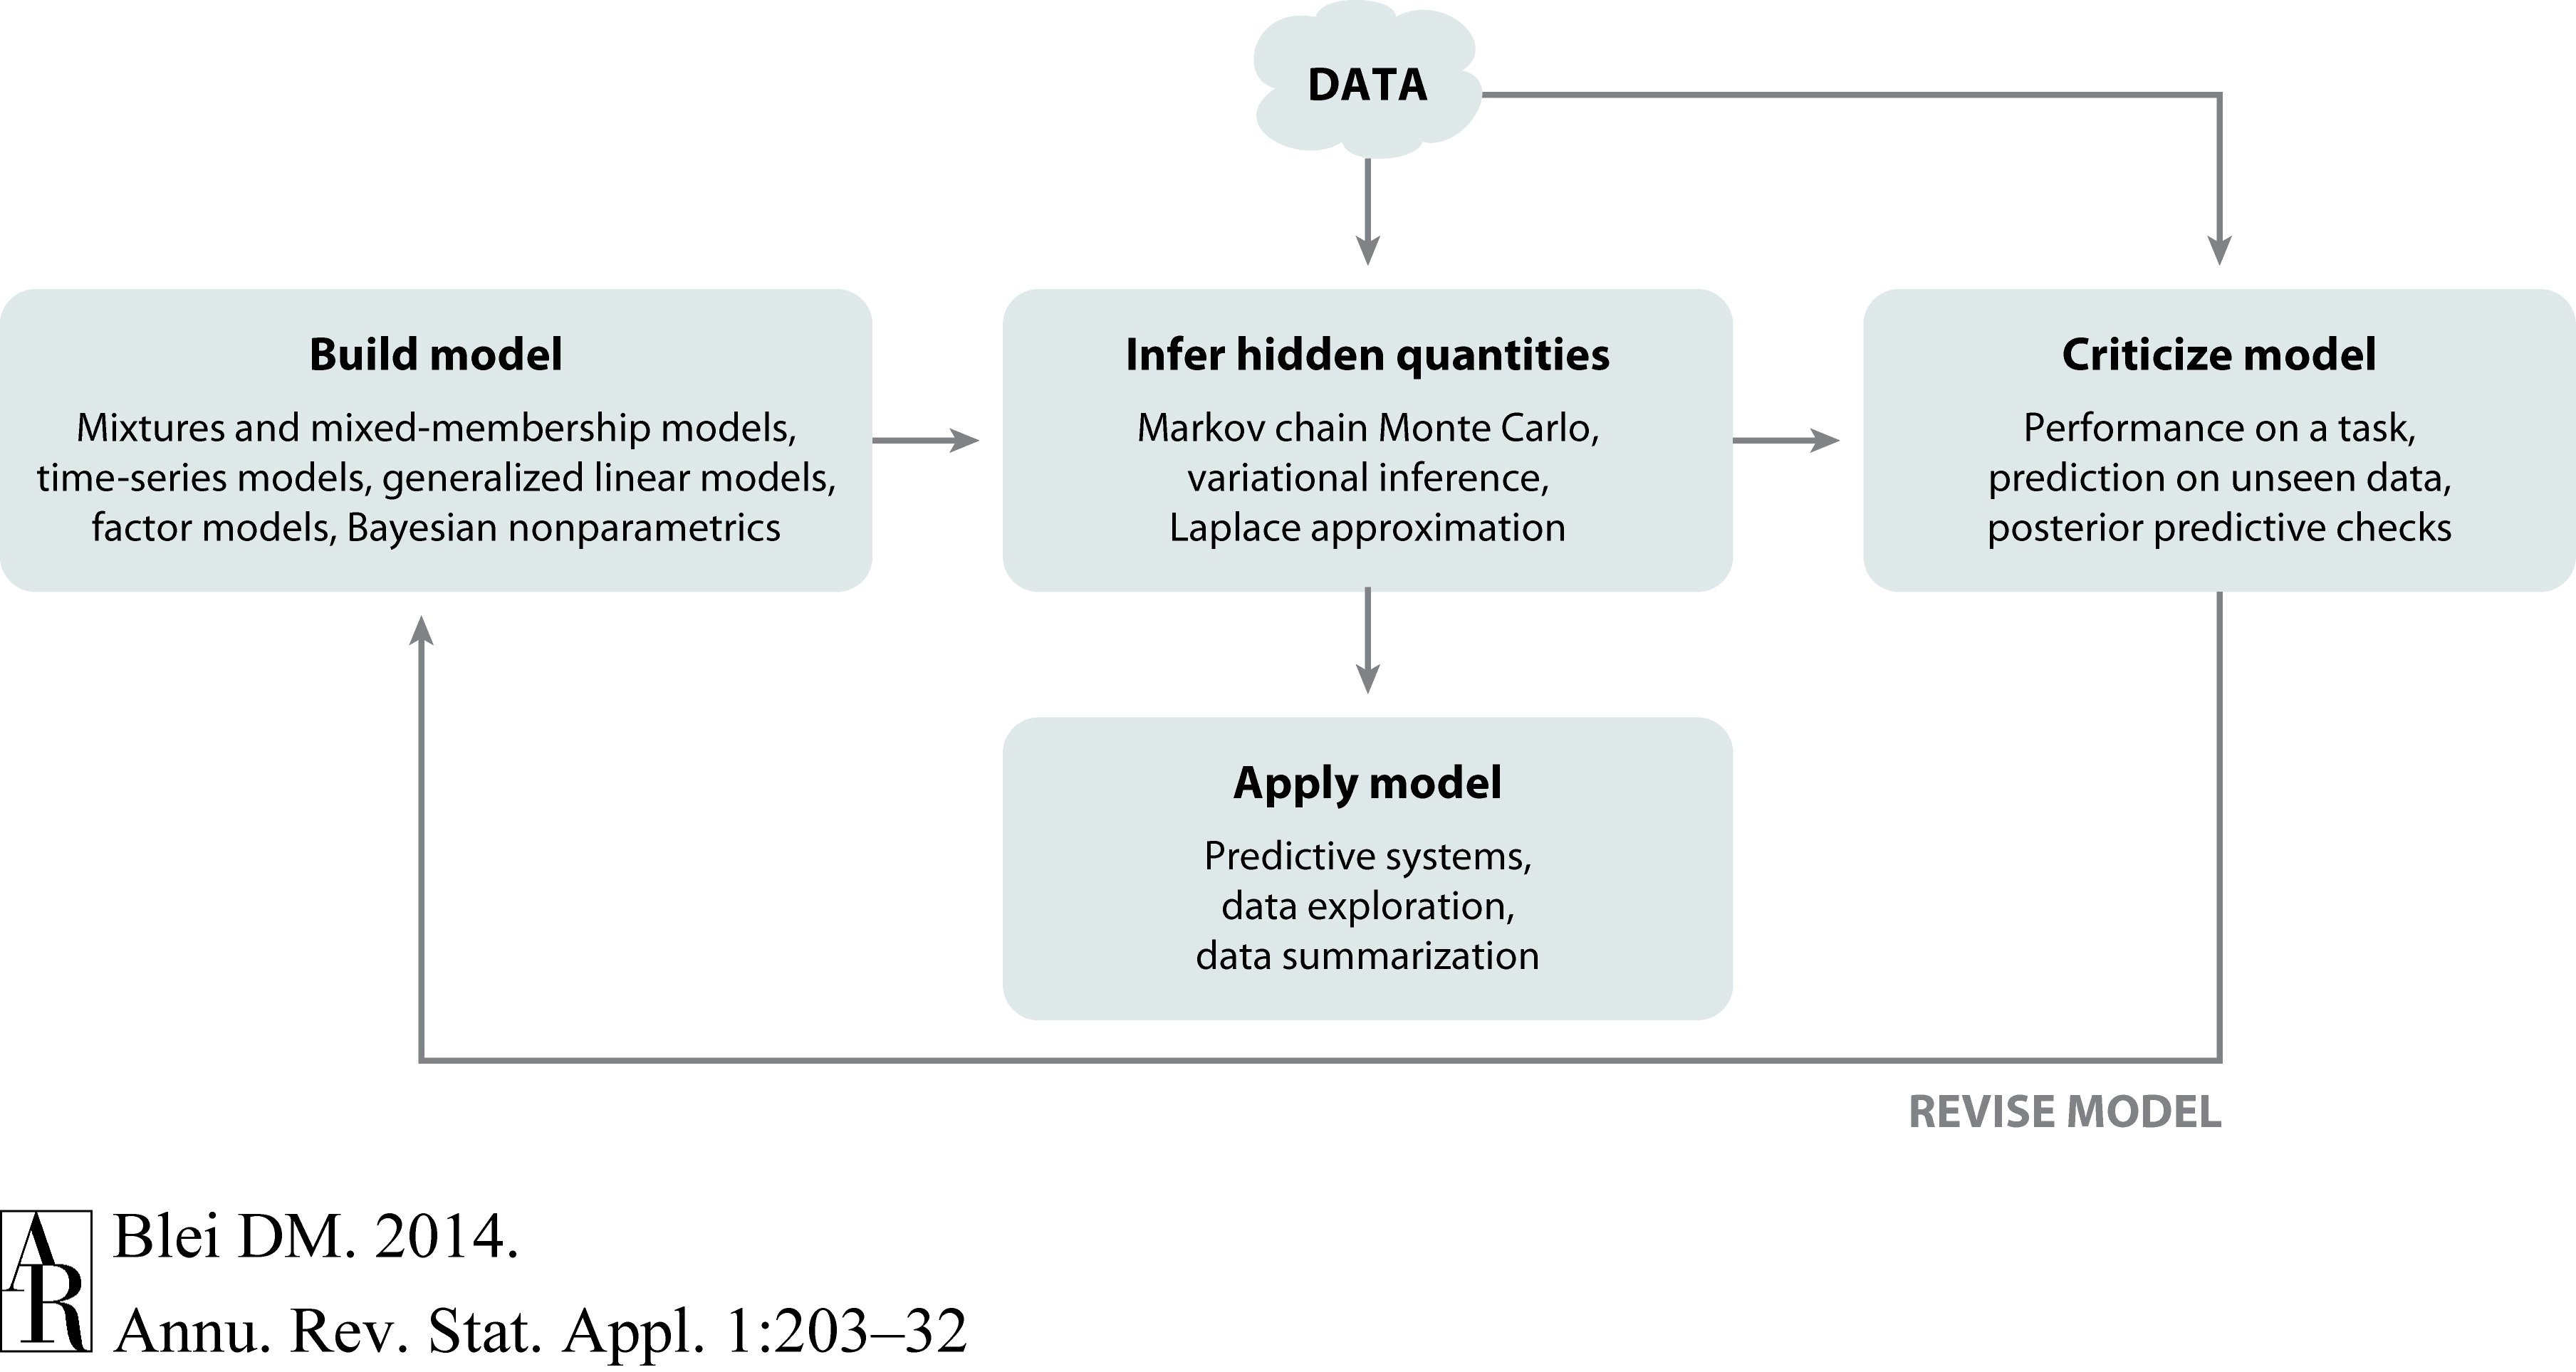
\includegraphics[width=.85\linewidth]{figures/lap1/boxsloop.jpeg}\\
\end{center} 
\begin{flushright}
{\footnotesize Blei, \textit{Ann. Rev. Stat. App.} 2014.}
\end{flushright}
\end{frame}

% \begin{frame}{Lap 7: Hidden Markov Models and Message Passing}
% \begin{itemize}
%     % \item \hyperref[sec:hmms]{\textbf{Model:} Hidden Markov Models}
%     \item \hyperref[sec:mp]{\textbf{Algorithm:} Message Passing}
% \end{itemize}
% \end{frame}

% \section{Model: HMMs}
% \label{sec:hmms}

\begin{frame}{Hidden Markov Models}

Hidden Markov Models (HMMs) assume a particular factorization of the joint distribution on latent states ($z_t$) and observations $(\mbx_t)$. The graphical model looks like this:

\begin{center}
    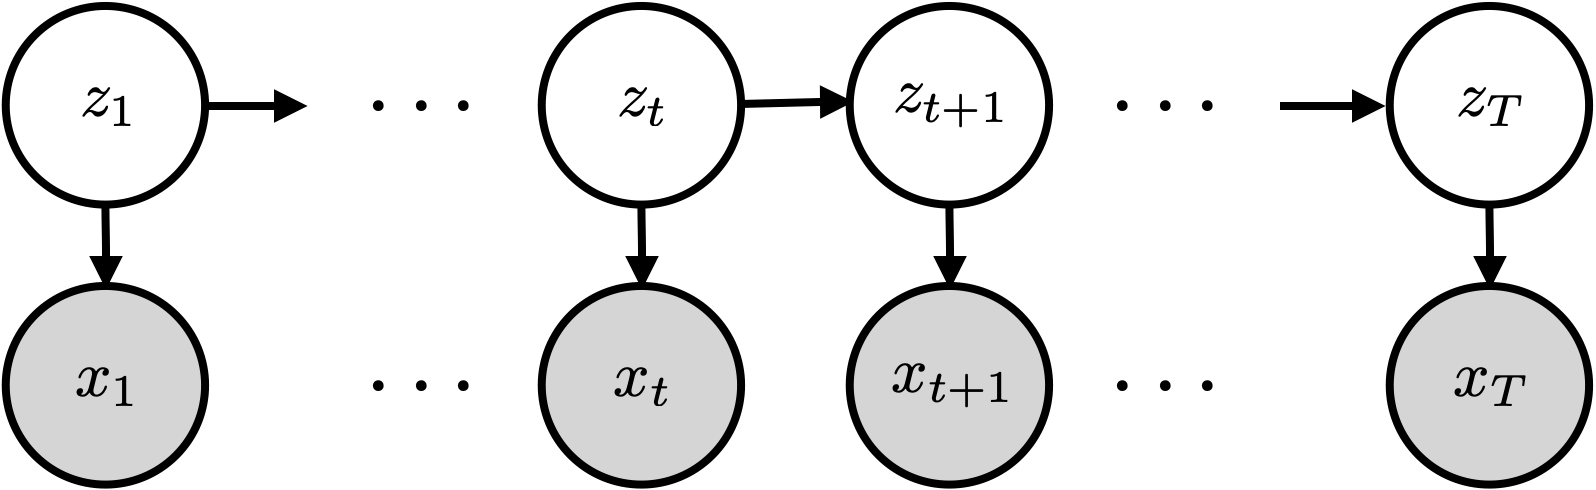
\includegraphics[width=0.7\textwidth]{figures/lap7/hmm.png}    
\end{center}

This graphical model says that the joint distribution factors as,
\begin{align}
    p(z_{1:T}, \mbx_{1:T}) &= p(z_1) \prod_{t=2}^T p(z_t \mid z_{t-1}) \prod_{t=1}^T p(\mbx_t \mid z_t).
\end{align}

We call this an HMM because $p(z_1) \prod_{t=2}^T p(z_t \mid z_{t-1})$ is a Markov chain.
    
\end{frame}

\begin{frame}{Hidden Markov Models II}
We are interested in questions like:
\begin{itemize}
    \item What is the \textit{posterior marginal} distribution $p(z_t \mid \mbx_{1:T})$?
    \item What is the \textit{posterior pairwise marginal} distribution $p(z_t, z_{t+1} \mid \mbx_{1:T})$?
    \item What is the \textit{posterior mode} $z_{1:T}^\star = \argmax p(z_{1:T} \mid \mbx_{1:T})$?
    \item What is the \textit{predictive distribution} of $p(z_{T+1} \mid \mbx_{1:T})$?
\end{itemize}

\end{frame}


\begin{frame}{State space models}
Note that nothing above assumes that $z_t$ is a discrete random variable!

HMM's are a special case of more general \textbf{state space models} with discrete states. 

State space models assume the same graphical model but allow for arbitrary types of latent states. 

For example, suppose that $\mbz_t \in \mathbb{R}^P$ are continuous valued latent states and that,
\begin{align}
    p(\mbz_{1:T}) &= p(\mbz_1) \prod_{t=2}^T p(\mbz_t \mid \mbz_{t-1}) \\
    &= \cN(\mbz_1 \mid \mbb_1, \mbQ_1) \prod_{t=2}^T \cN(\mbz_t \mid \mbA \mbz_{t-1} + \mbb, \mbQ) 
\end{align}
This is called a \textbf{linear dynamical system} with Gaussian noise. 

\end{frame}

\begin{frame}{Message passing in HMMs}

In the HMM with discrete states, we showed how to compute posterior marginal distributions using message passing,
\begin{align}
    p(z_t \mid \mbx_{1:T}) &\propto \sum_{z_1} \cdots \sum_{z_{t-1}} \sum_{z_{t+1}} \cdots \sum_{z_T} p(z_{1:T}, \mbx_{1:T}) \\
    &= \alpha_t(z_t) \, p(\mbx_t \mid z_t) \, \beta_t(z_t) 
\end{align}
where the \textit{forward and backward messages} are defined recursively
\begin{align}
    \alpha_t(z_t) &= \sum_{z_{t-1}} p(z_t \mid z_{t-1}) \, p(\mbx_{t-1} \mid z_{t-1}) \, \alpha_{t-1}(z_{t-1}) \\
    \beta_t(z_t) &= \sum_{z_{t+1}} \, p(z_{t+1} \mid z_t) \, p(\mbx_{t+1} \mid z_{t+1}) \, \beta_{t+1}(z_{t+1})
\end{align}
The initial conditions are $\alpha_1(z_1) = p(z_1)$ and $\beta_{T}(z_T) = 1$.
    
\end{frame}

\begin{frame}{What do the forward messages tell us?}
\label{slide:fwd_hmm}

The forward messages are equivalent to,
\begin{align}
    \alpha_t(z_t) &= \sum_{z_1} \cdots \sum_{z_{t-1}} p(z_{1:t}, \mbx_{1:t-1}) \\
    &p(z_t, \mbx_{1:t-1}).
\end{align}
The normalized message is the \textit{predictive distribution},
\begin{align}
    \frac{\alpha_t(z_t)}{\sum_{z_t'} \alpha_t(z_t')} &= 
    \frac{p(z_t, \mbx_{1:t-1})}{\sum_{z_t'} p(z_t', \mbx_{1:t-1})} = \frac{p(z_t, \mbx_{1:t-1})}{p(\mbx_{1:t-1})} = p(z_t \mid \mbx_{1:t-1}),
\end{align}
The final normalizing constant yields the marginal likelihood, $\sum_{z_T} \alpha_T(z_T) = p(\mbx_{1:T})$.

% Here, $z_t$ is a discrete random variable so we can think of the message as a vector,
% \begin{align}
%     \mbalpha_t &= [\alpha_{t1}, \ldots, \alpha_{tK}]^\top,
% \end{align}
% with  $\alpha_t(z_t)$ pulling out the $z_t$-th entry in this vector.

\end{frame}

\begin{frame}{Message passing in state space models}

The same recursive algorithm applies (in theory) to any state space model with the same factorization, but the sums are replaced with integrals,
\begin{align}
    p(z_t \mid \mbx_{1:T}) &\propto \int \dif z_1 \cdots \int \dif {z_{t-1}} \int \dif{z_{t+1}} \cdots \int \dif {z_T} \,  p(z_{1:T}, \mbx_{1:T}) \\
    &= \alpha_t(z_t) \, p(\mbx_t \mid z_t) \, \beta_t(z_t) 
\end{align}
where the \textit{forward and backward messages} are defined recursively
\begin{align}
    \alpha_t(z_t) &= \int p(z_t \mid z_{t-1}) \, p(\mbx_{t-1} \mid z_{t-1}) \, \alpha_{t-1}(z_{t-1}) \dif {z_{t-1}} \\
    \beta_t(z_t) &= \int p(z_{t+1} \mid z_t) \, p(\mbx_{t+1} \mid z_{t+1}) \, \beta_{t+1}(z_{t+1}) \dif {z_{t+1}} 
\end{align}
The initial conditions are $\alpha_1(z_1) = p(z_1)$ and $\beta_{T}(z_T) = 1$.
    
\end{frame}

\begin{frame}[t]{Message passing in a linear dynamical system}
\textbf{Exercise:} Consider an LDS with Gaussian noise and assume that $p(\mbx_t \mid \mbz_t) = \cN(\mbx_t \mid \mbC \mbz_t + \mbd, \mbR)$. Derive the forward message $\alpha_t(\mbz_t)$ under the inductive hypothesis that $\alpha_{t-1}(\mbz_{t-1}) \propto \cN(\mbz_{t-1} \mid \mbmu_{t-1}, \mbSigma_{t-1})$.
\end{frame}

\begin{frame}[t]{Message passing in nonlinear dynamical systems}
\textbf{Question:} What if $p(\mbz_t \mid \mbz_{t-1}) = \cN(z_t \mid f(\mbz_{t-1}), \mbQ)$ for some nonlinear function $f$? 

\end{frame}

\begin{frame}{Sequential Monte Carlo}
Recall that the forward messages are proportional to the predictive distributions $p(\mbz_t \mid \mbx_{1:t-1})$. We can view the forward recursions as an expectation,
\begin{align}
    \alpha_t(\mbz_t) &= \int p(\mbz_t \mid z_{t-1}) \, p(\mbx_{t-1} \mid \mbz_{t-1}) \, \alpha_{t-1}(\mbz_{t-1}) \dif {\mbz_{t-1}} \\
    &\propto \E_{\mbz_{t-1} \sim p(\mbz_{t-1} \mid \mbx_{1:t-2})} \left[ p(\mbz_t \mid z_{t-1}) \, p(\mbx_{t-1} \mid \mbz_{t-1}) \right] 
\end{align}
One natural idea is to approximate this expectation with Monte Carlo,
\begin{align}
    \hat{\alpha}_t(\mbz_t) 
    &\approx \frac{1}{S} \sum_{s=1}^S \left[ w_{t-1}^{(s)} \, p(\mbz_t \mid \mbz_{t-1}^{(s)})  \right] 
\end{align}
where we have defined the \textbf{weights} $w_{t-1}^{(s)} \triangleq p(\mbx_{t-1} \mid \mbz_{t-1}^{(s)})$.

How do we sample $\mbz_{t-1}^{(s)} \iid{\sim} p(\mbz_{t-1} \mid \mbx_{1:t-2})$? Let's sample the normalized $\hat{\alpha}_{t-1}(\mbz_{t-1})$ instead!
\end{frame}

\begin{frame}{Sequential Monte Carlo II}
The normalizing constant is,
\begin{align}
   \int \hat{\alpha}_{t-1}(\mbz_{t-1}) \dif \mbz_{t-1} &= 
   \frac{1}{S} \sum_{s=1}^S w_{t-2}^{(s)} \int p(\mbz_{t-1} \mid \mbz_{t-2}^{(s)}) \dif \mbz_{t-1} 
   = \frac{1}{S} \sum_{s=1}^S w_{t-2}^{(s)}.
\end{align}
Use this to define the \textit{normalized forward message} (i.e. the Monte Carlo estimate of the predictive distribution) is,
\begin{align}
    \bar{\alpha}_{t-1}(\mbz_{t-1}) &\triangleq \frac{\hat{\alpha}_{t-1}(\mbz_{t-1})}{\int \hat{\alpha}_{t-1}(\mbz_{t-1}') \dif \mbz_{t-1}'}
    = \sum_{s=1}^S \bar{w}_{t-2}^{(s)} \, p(\mbz_{t-1} \mid \mbz_{t-2}^{(s)})
\end{align}
where $\bar{w}_{t-2}^{(s)} = \frac{w_{t-2}^{(s)}}{\sum_{s'} w_{t-2}^{(s')}}$ is the normalized weight of sample $\mbz_{t-2}^{(s)}$.

\textbf{The normalized forward message is just a mixture distribution with weights $\bar{w}_{t-2}^{(s)}$!}
\end{frame}

\begin{frame}{Putting it all together}
Combining the above, we have the following algorithm for the forward pass:
\begin{enumerate}
    \item Let $\bar{\alpha}_1(\mbz_1) = p(z_1)$
    \item For $t=1, \ldots, T$:
    \begin{enumerate}[a.]
        \item Sample $\mbz_{t}^{(s)} \iid{\sim} \bar{\alpha}_t(\mbz_t)$ for $s=1, \ldots, S$
        \item Compute weights $w_t^{(s)} = p(\mbx_t \mid \mbz_t^{(s)})$ and normalize $\bar{w}_t^{(s)} = w_t^{(s)} / \sum_{s'} w_t^{(s')}$.
        \item Compute normalized forward message $\bar{\alpha}_{t+1}(\mbz_{t+1}) = \sum_{s=1}^S \bar{w}_t^{(s)} p(\mbz_{t+1} \mid \mbz_t^{(s)})$.
    \end{enumerate}
\end{enumerate}

This is called \textbf{sequential Monte Carlo} (SMC) using the model dynamics as the proposal.

Note that Step 2a can \textbf{resample} the same $\mbz_{t-1}^{(s)}$ multiple times according to its weight. 

\textbf{Question:} How can you approximate the marginal likelihood $p(\mbx_{1:T})$ using the weights? \textit{Hint: look back to Slide~\ref{slide:fwd_hmm}}.

\end{frame}

\begin{frame}{Generalizations}
    \begin{itemize}
        \item Instead of sampling $\bar{\alpha}_{t}(\mbz_{t})$, we could have sampled with a \textbf{proposal distribution} $r(\mbz_{t} \mid \mbz_{t-1}^{(s)})$ instead and corrected for it by defining the weights to be,
        \begin{align}
            w_t^{(s)} &= \frac{p(\mbz_{t} \mid \mbz_{t-1}^{(s)}) \, p(\mbx_t \mid \mbz_t)}{r(\mbz_{t} \mid \mbz_{t-1}^{(s)})}
        \end{align}
        Moreover, the proposal distribution can ``look ahead'' to future data $\mbx_t$.
    \end{itemize}
\end{frame}

\begin{frame}[t,allowframebreaks]
        \frametitle{References}
        \bibliographystyle{unsrtnat}
        \bibliography{refs.bib}
\end{frame}

\end{document}